\documentclass[
	aspectratio=169, % default is 43
	8pt, % font size, default is 11pt
	handout, % handout mode without animations, comment out to add animations
]{beamer}
\def\university{}

\documentclass[
	aspectratio=169, % default is 43
	8pt, % font size, default is 11pt
	handout, % handout mode without animations, comment out to add animations
]{beamer}

\usepackage{../template/beamerthemeuulm} % use the inofficial uulm beamer theme
\setfaculty{infIngPsy} % set the color scheme for your faculty here [med/infIngPsy/math/nat]

% requires symbolic links
% git clone git@github.com:SoftVarE-Group/SlideTemplate.git C:\Users\...\SlideTemplate
% mklink /J template C:\Users\...\SlideTemplate
% git clone git@spgit.informatik.uni-ulm.de:thuem/slides.git C:\Users\...\ThomasSlides
% mklink /J thomasslides C:\Users\...\ThomasSlides
\graphicspath{{../template/pics/logos}{../template/pics/nature}{../template/pics/uulm}{../thomasslides/}{../pics/}}

%\usepackage[ngerman]{babel} % use this line for slides in German
%\recordingtrue % special recording mode for use with a greenscreen, gives you space to show yourself in a layer in front of the slides, has no effect in the handout mode

\title{Software Product Lines} % short title is used for the slide footer but optional

%
%
%% IMPORTED PACKAGES
%
%\usepackage{adjustbox} % used for partofpage
%\usepackage{tcolorbox} % used for mydefinition, mynote, myexample
\usepackage{multicol} % used temporarily for the lecture overview
%\usepackage{mathtools} % required for absolute value in modeling lecture
%
%% SLIDE TEMPLATE
%
%\beamertemplatenavigationsymbolsempty 
%
%% COMMANDS TO LAYOUT AND ANNIMATE SLIDES
%
\newcommand{\lessonslearned}[3]{
	\subsection{Summary}
	\begin{frame}{\insertsection -- \insertsubsection}
		\leftorright{
			\mydefinition{Lessons Learned}{
				\begin{itemize}
					#1
				\end{itemize}
			}
			\mynote{Further Reading}{
				\small % references take space, can be a little smaller
				\begin{itemize}
					#2
				\end{itemize}
			}
		}{
			\myexample{Practice}{
				#3
			}
		}
	\end{frame}
}

\renewcommand{\lectureoverview}{
%	\section*{Overview}
%	\subsection*{Overview}
	\begin{frame}{\insertsubtitle}
		\begin{multicols}{2}
			\tableofcontents
		\end{multicols}
	\end{frame}
}

%
%\newcommand{\onlyleft}[1]{
%	\halfpage{#1}
%}
%
%\newcommand{\onlyright}[1]{
%	~\hfill
%	\halfpage{#1}
%}
%
%\newcommand{\leftorright}[2]{
%	\uncover<1>{\halfpage{#1}}
%	\hfill
%	\uncover<3->{\halfpage{#2}}
%}
%
%\newcommand{\rightorleft}[2]{
%	\uncover<3->{\halfpage{#1}}
%	\hfill
%	\uncover<1>{\halfpage{#2}}
%}
%
%\newcommand{\leftthenright}[2]{
%	\halfpage{#1}
%	\hfill\pause
%	\halfpage{#2}
%}
%
%\newcommand{\leftandright}[2]{
%	\halfpage{#1}
%	\hfill
%	\halfpage{#2}
%}
%
%\newcommand{\leftmiddleandright}[3]{
%	\thirdpage{#1}
%	\hfill
%	\thirdpage{#2}
%	\hfill
%	\thirdpage{#3}
%}
%
%\newcommand{\leftmiddleorright}[3]{
%	\uncover<1>{\thirdpage{#1}}
%	\hfill
%	\uncover<3>{\thirdpage{#2}}
%	\hfill
%	\uncover<5->{\thirdpage{#3}}
%}
%
%\newcommand{\halfpage}[1]{\partofpage{48}{#1}}
%
%\newcommand{\thirdpage}[1]{\partofpage{31}{#1}}
%
%\newcommand{\partofpage}[2]{
%	\adjustbox{valign=t}{\begin{minipage}{0.#1\textwidth}
%			\begin{flushleft}
%				#2
%			\end{flushleft}
%	\end{minipage}}
%}
%
%\newcommand{\mydefinition}[2]{
%	\begin{tcolorbox}[title=#1,colback=orange!10,colframe=orange!30,coltitle=black,fonttitle=\bfseries,left=1mm,right=1mm,top=1mm,bottom=1mm]
%		\begin{flushleft}
%			#2
%		\end{flushleft}
%	\end{tcolorbox}
%}
%
%\newcommand{\mydefinitiontight}[2]{
%	\begin{tcolorbox}[title=#1,colback=white,colframe=orange!30,coltitle=black,fonttitle=\bfseries,left=0mm,right=0mm,top=0mm,bottom=0mm]
%		\begin{flushleft}
%			#2
%		\end{flushleft}
%	\end{tcolorbox}
%}
%
%\newcommand{\mynote}[2]{
%	\begin{tcolorbox}[title=#1,colback=red!10,colframe=red!30,coltitle=black,fonttitle=\bfseries,left=1mm,right=1mm,top=1mm,bottom=1mm]
%		\begin{flushleft}
%			#2
%		\end{flushleft}
%	\end{tcolorbox}
%}
%
%\newcommand{\myexample}[2]{
%	\begin{tcolorbox}[title=#1,colback=blue!10,colframe=blue!30,coltitle=black,fonttitle=\bfseries,left=1mm,right=1mm,top=1mm,bottom=1mm]
%		\begin{flushleft}
%			#2
%		\end{flushleft}
%	\end{tcolorbox}
%}
%
%\newcommand{\myexampletight}[2]{
%	\begin{tcolorbox}[title=#1,colback=white,colframe=blue!30,coltitle=black,fonttitle=\bfseries,left=0mm,right=0mm,top=0mm,bottom=0mm]
%		\begin{flushleft}
%			#2
%		\end{flushleft}
%	\end{tcolorbox}
%}

\subtitle{10. Product-Line Analyses}
\author{Elias Kuiter, Thomas Thüm, Timo Kehrer}
\foruniversity{}
	{
		%\setpicture[50]{ovgu-autumn3}\setcopyright{Photo: Hannah Theile (OVGU)} % add new picuter
	}
	{\setpicture{oct20-south4}}

\usepackage{algpseudocode}

\begin{document}

% TITLE SLIDE

\maketitle

% SLIDE TEMPLATE

%\setbeamercolor{title}{fg=black}
%\setbeamercolor{frametitle}{fg=black}
\setbeamertemplate{frametitle}{{\huge~\\\insertsubsection~\insertframetitle}}
\setbeamertemplate{footline}[text line]{\parbox{\linewidth}{\vspace*{-10pt}\hspace{0pt}%
	\insertshortauthor\phantom{g\insertpagenumber}%
	\hfill%
	\inserttitle%
	\ifx \insertsubtitle \empty \else \ -- \insertsubtitle\fi%
	\ifx \insertsectionhead \empty \else \ -- \insertsectionhead\fi%
	\hfill%
	\phantom{g\insertshortauthor}\insertpagenumber%
}}
%\defbeamertemplate{footline}{\begin{beamercolorbox}[sep=1em]{author in head/foot}\insertshortauthor\hfill\insertsection\hfill\insertframenumber\end{beamercolorbox}}
%\defbeamertemplate*{footline}{mytheme}{\begin{beamercolorbox}[sep=1em]{author in head/foot}\insertshortauthor\hfill\insertsection\hfill\insertframenumber\end{beamercolorbox}}

% OVERVIEW SLIDES

\newcommand{\overview}{
	\section*{Overview}
	\subsection*{Overview}
	\begin{frame}{-- \insertsubtitle}
		\begin{multicols}{3}
			\tableofcontents
		\end{multicols}
	
		\begin{flushright}
			\footnotesize
			Author: \insertauthor
			
			Date: \insertdate
		\end{flushright}
	\end{frame}
}
% temporarily added slide to have a lecture overview 
\overview

% temporarily removed
%\begin{frame}{Lecture Overview -- \insertsubtitle}
%	\tableofcontents[hideallsubsections]
%\end{frame}

\AtBeginSection[]{%
	\begin{frame}{Lecture Overview -- \insertsubtitle}
		\tableofcontents[currentsection,hideothersubsections]
	\end{frame}
}

\newcommand{\sectionend}{\addtocontents{toc}{\newpage}}


\section{Analysis Strategies}

\newcommand{\pluseq}{\mathrel{+}=}

\newcommand{\familybasedlego}{
	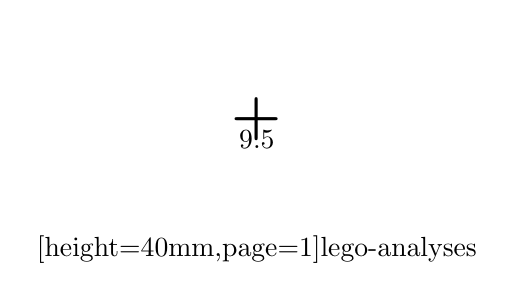
\begin{tikzpicture}
		\node (lego) at (0,-1.7) {\pic[height=40mm,page=1]{lego-analyses}};
		\node (lego) at (0,-.05) {\huge \textbf{+}};
		\node (lego) at (0,1) {\footnotesize\featureDiagramLego};
		\node at (0,-.3) {\mglass{9.5}};
	\end{tikzpicture}
}

\newcommand{\summaryproductbased}{
	\centering\pic[width=.8\linewidth,page=9]{lego-analyses}
	\mynote{Product-Based Strategy}{
		\begin{itemize}
			\item analyze individual \emph{products}
			\item[+] sound, complete
			\item[+] uses off-the-shelf generator\,$\gamma$ and analysis\,$\alpha$
			\item[--] redundant effort
			\item[--] does not scale well
		\end{itemize}
	}
}

\newcommand{\summaryfeaturebased}{
	\centering\pic[width=.8\linewidth,page=6]{lego-analyses}
	\mynote{Feature-Based Strategy}{
		\begin{itemize}
			\item analyze individual \emph{features}
			\item[+] sound, efficient
			\item[--] analysis $\alpha$ requires features with interfaces
			\item[--] incomplete: misses all feature interactions
		\end{itemize}
	}
}

\newcommand{\summaryfamilybased}{
	\centering\scalebox{.5}{\familybasedlego}
	\mynote{Family-Based Strategy}{
		\begin{itemize}
			\item analyze the \emph{product line}
			\item[+] sound, complete, efficient
			\item[--] requires careful, hand-crafted analysis $\alpha$
		\end{itemize}
	}
}

\subsection{Recap: Quality Assurance}

\begin{frame}{\myframetitle\ \mytitlesource{\ludewiglichter}}
	\begin{mycolumns}[widths={45},animation=none]
		\uncover<2->{\mynote{}{
			\begin{itemize}
				\item last lecture:\\
					how to \emph{avoid} variability bugs (esp. feature interactions)
				\uncover<4->{\item this + next lecture:\\
					how to \emph{find} variability bugs}
			\end{itemize}
		}}
	\mynextcolumn
		\only<1|handout:0>{\includegraphics[height=\textheightwithtitle,page=1]{quality-assurance}}%
		\only<2|handout:0>{\includegraphics[height=\textheightwithtitle,page=2]{quality-assurance}}%
		\only<3|handout:0>{\includegraphics[height=\textheightwithtitle,page=3]{quality-assurance}}%
		\only<4|handout:0>{\includegraphics[height=\textheightwithtitle,page=4]{quality-assurance}}%
		\only<5|handout:1>{\includegraphics[height=\textheightwithtitle,page=5]{quality-assurance}}%
		\only<6|handout:0>{\includegraphics[height=\textheightwithtitle,page=6]{quality-assurance}}%
	\end{mycolumns}
\end{frame}

\widexkcdframe{1700}

\subsection{Automated Analysis of Product Lines}

\begin{frame}{\myframetitle}
	\begin{mycolumns}[t,widths={47}]
		\mynote{Typical Program Analyses}{
			\leftandright{
				\begin{itemize}
					\item code metrics
					\item type checking
					\item theorem proving
					\item data-flow analysis
					\item performance analysis
					\item \ldots
				\end{itemize}
			}{
				\hspace*{10mm}\mglass{3}
			}
		}
		\mydefinition{What is a Program Analysis?}{
			\begin{itemize}
				\item analyzes properties of a \emph{program} (e.g., correctness, performance, and safety)
				\item can be used to automatically find bugs, bottlenecks, and other \emph{vulnerabilities}
			\end{itemize}
		}
		\mynextcolumn
		\myexample{Asking Questions About Product Lines}{
			\begin{itemize}
				\item Which product has the most lines of code? \mysource{\href{https://dl.acm.org/doi/10.1145/3307630.3342384}{ref}}
				\item Which products have type errors? \mysource{\href{https://dl.acm.org/doi/10.1145/1868688.1868693}{ref}}
				\item Which products violate specifications? \mysource{\href{https://dl.acm.org/doi/10.1145/2371401.2371404}{ref}}
				\item Which products have unsafe data flows? \mysource{\href{https://dl.acm.org/doi/10.1145/2499370.2491976}{ref}}
				\item Which is the fastest product? \mysource{\href{https://link.springer.com/article/10.1007/s10515-020-00273-8}{ref}}\\
					Which product has the smallest binary? \mysource{\href{https://dl.acm.org/doi/10.1145/3546932.3546997}{ref}}
				\item \ldots
			\end{itemize}
		}
		\mydefinition{What is a Product-Line Analysis?}{
			\begin{itemize}
				\item analyzes properties of an entire \emph{product line}
				\item can be roughly classified by its \emph{strategy}:
				\begin{itemize}
					\item product-based
					\item feature-based
					\item family-based
				\end{itemize}
			\end{itemize}
		}
	\end{mycolumns}
\end{frame}

\subsection{Product-Based Strategies} % refs missing in whole part!

\begin{frame}{\myframetitle}
	\begin{mycolumns}
		\mydefinition{Intuition}{
			\begin{itemize}
				\item to analyze the product line, just analyze \emph{each product}
				\begin{itemize}
					\item individually
					\item in isolation
					\item possibly in parallel
				\end{itemize}
				\item e.g., compile and verify each product
			\end{itemize}
		}
		\myexampletight{}{\centering\featureDiagramLego\\$Helmet \pimplies \pnot Phone$}
	\mynextcolumn
		\pic[width=\linewidth,page=9]{lego-analyses}
	\end{mycolumns}
\end{frame}

\begin{frame}{\myframetitle}
	\begin{mycolumns}
		\mydefinition{Algorithm}{
			\begin{algorithmic}
				\Require a product line $pl$; algorithms $\gamma$, $\alpha$, $\sigma$
				\State $C \gets AllSAT(\phi(FM_{pl}))$ \Comment{{\small enumerate valid config's}}
				\State $results \gets []$
				\ForAll{$S \in C$} \Comment{{\small for each valid config}}
				\State $p \gets \gamma(S)$ \Comment{{\small generate product}}
				\State $results \pluseq \alpha(p)$ \Comment{{\small add analysis result}}
				\EndFor
				\State \Return $\sigma(results)$
			\end{algorithmic}
		}
		\mynote{}{
			\begin{itemize}
				\item $\gamma$ \emph{generates} (e.g., compiles) products (e.g., \texttt{make}, \texttt{gradle}, \texttt{FeatureHouse}, \texttt{npm}, \ldots)
				\item $\alpha$ \emph{analyzes} the product (e.g., run verifier)
				\item $\sigma$ \emph{summarizes} the results (e.g., each individual call to $\alpha$ must succeed)
			\end{itemize}
		}
	\mynextcolumn
		\myexampletight{}{
			\begin{center}
				\small\featureDiagramConfigurableDatabase
			\end{center}
		}
		\myexample{}{
			\footnotesize
			\leftandright{
				$\sigma([\alpha(\gamma(\{C,G,W\}))$\\
				$~~~~\alpha(\gamma(\{C,P,W\}))$\\
				$~~~~\alpha(\gamma(\{C,G,P,W\}))$\\
				$~~~~\alpha(\gamma(\{C,D,W\}))$\\
				$~~~~\alpha(\gamma(\{C,G,D,W\}))$\\
				$~~~~\alpha(\gamma(\{C,P,D,W\}))$\\
				$~~~~\alpha(\gamma(\{C,G,P,D,W\}))$\\
				$~~~~\alpha(\gamma(\{C,P,T,W\}))$\\
				$~~~~\alpha(\gamma(\{C,G,P,T,W\}))$\\
				$~~~~\alpha(\gamma(\{C,D,T,W\}))$\\
				$~~~~\alpha(\gamma(\{C,G,D,T,W\}))$\\
				$~~~~\alpha(\gamma(\{C,P,D,T,W\}))$\\
				$~~~~\alpha(\gamma(\{C,G,P,D,T,W\}))$
			}{
				$\alpha(\gamma(\{C,G,L\}))$\\
				$\alpha(\gamma(\{C,P,L\}))$\\
				$\alpha(\gamma(\{C,G,P,L\}))$\\
				$\alpha(\gamma(\{C,D,L\}))$\\
				$\alpha(\gamma(\{C,G,D,L\}))$\\
				$\alpha(\gamma(\{C,P,D,L\}))$\\
				$\alpha(\gamma(\{C,G,P,D,L\}))$\\
				$\alpha(\gamma(\{C,P,T,L\}))$\\
				$\alpha(\gamma(\{C,G,P,T,L\}))$\\
				$\alpha(\gamma(\{C,D,T,L\}))$\\
				$\alpha(\gamma(\{C,G,D,T,L\}))$\\
				$\alpha(\gamma(\{C,P,D,T,L\}))$\\
				$\alpha(\gamma(\{C,G,P,D,T,L\}))])$
			}
		}
	\end{mycolumns}
\end{frame}

\begin{frame}{Classification of Strategies}
	\begin{mycolumns}[t,columns=3,animation=none]
		\summaryproductbased
	\mynextcolumn
	\mynextcolumn
	\end{mycolumns}
\end{frame}

\subsection{Feature-Based Strategies}

\begin{frame}{\myframetitle}
	\begin{mycolumns}
		\mydefinition{Intuition}{
			\begin{itemize}
				\item to analyze the product line, just analyze \emph{each feature} individually
				\item ignore all relations to other features
				\item e.g., compile and verify each component\\
				$\Rightarrow$ requires \emph{interfaces between features} (components, services, plug-ins) % todo: rename lecture 6 accordingly?
			\end{itemize}
		}
		\myexampletight{}{\centering\featureDiagramLego\\$Helmet \pimplies \pnot Phone$}
	\mynextcolumn
		\pic[width=\linewidth,page=6]{lego-analyses}
	\end{mycolumns}
\end{frame}

\begin{frame}{\myframetitle}
	\begin{mycolumns}
		\mydefinition{Algorithm}{
			\begin{algorithmic}
				\Require a product line $pl$; algorithms $\alpha$, $\sigma$
				\State $results \gets []$
				\ForAll{$f \in F_{pl}$} \Comment{{\small for each feature}}
				\State $results \pluseq \alpha(f)$ \Comment{{\small add analysis result}}
				\EndFor
				\State \Return $\sigma(results)$
			\end{algorithmic}
		}
		\mynote{}{
			\begin{itemize}
				\item $\alpha$ \emph{analyzes} the feature (e.g., compiles and verifies the component)
				\item $\sigma$ \emph{summarizes} the results (see product-based)
			\end{itemize}
		}
	\mynextcolumn
		\myexampletight{}{
			\begin{center}
				\small\featureDiagramConfigurableDatabase
			\end{center}
		}
		\myexample{}{
			\vspace*{-4ex}
			\small
			\begin{align*}
				\sigma([&\alpha(\gamma(C)) \text{ -- e.g., compile and verify base code}\\
				&\alpha(\gamma(G)) \text{ -- e.g., compile and verify feature Get}\\
				&\alpha(\gamma(P)) \text{ -- \ldots}\\
				&\alpha(\gamma(D))\\
				&\alpha(\gamma(T))\\
				&\alpha(\gamma(W))\\
				&\alpha(\gamma(L))])
			\end{align*}
		}
	\end{mycolumns}
\end{frame}

\begin{frame}{Classification of Strategies}
	\begin{mycolumns}[t,columns=3,animation=none]
		\summaryproductbased
	\mynextcolumn
		\summaryfeaturebased
	\mynextcolumn
	\end{mycolumns}
\end{frame}

\subsection{Family-Based Strategies}

\begin{frame}{\myframetitle}
	\begin{mycolumns}
		\mydefinition{Intuition}{
			\begin{itemize}
				\item analyze the product line (or \emph{family}) as a whole
				\item requirement: the analysis should give the same result as a product-based analysis
				\item makes use of the feature model and artifacts
				\item analysis is \emph{hand-crafted}, no generic algorithm\\
				$\Rightarrow$ typically: reduction to SAT problems
			\end{itemize}
		}
		\myexample{Today's Examples}{
			\begin{itemize}
				\item analyzing \emph{feature mappings}
				\item analyzing \emph{variable code}
			\end{itemize}
			$\Rightarrow$ here: only for \emph{conditional compilation}
		}
	\mynextcolumn
		\centering\familybasedlego
	\end{mycolumns}
\end{frame}

\subsection{Classification of Strategies}

\begin{frame}{\myframetitle}
	\begin{mycolumns}[t,columns=3,animation=none]
		\summaryproductbased
	\mynextcolumn
		\summaryfeaturebased
	\mynextcolumn
		\summaryfamilybased
	\end{mycolumns}
\end{frame}

\lessonslearned{
	\item product-line analyses are needed for quality assurance
	\item \emph{product-based}: simple, but does not scale
	\item \emph{feature-based}: fairly simple, but misses interactions
	\item \emph{family-based}: efficient, but most complex
}{
	\item \fospl, Chapter 10
	\item \analysisstrategies
}{
	Can you imagine other analysis strategies than product-based, feature-based, and family-based?
	How could such strategies look like?
}

\sectionend

\section{Analyzing Feature Mappings}


\newcommand{\notleftright}{\mathrel{\ooalign{$\Leftrightarrow$\cr\hidewidth$/$\hidewidth}}}

\subsection{The Use of Feature-Mapping Analyses}

\begin{frame}{\myframetitle}
	\begin{mycolumns}[widths={45,55}]
		\mynote{Recap: A Typical Product Line}{
			\begin{itemize}
				\item embedded or systems programming (e.g., Linux)
				\item implemented with conditional compilation
				\begin{itemize}
					\item build systems (e.g., KBuild)
					\item preprocessors (e.g., CPP)
				\end{itemize}
				\item feature traceability only implicit\\
					$\Rightarrow$ there is code scattering and tangling
			\end{itemize}
		}
		\mydefinition{Recap: Feature Mapping}{
			\begin{itemize}
				\item \todots
			\end{itemize}
		}
		\mynextcolumn
		\myexample{Asking Questions About the Feature Mapping}{
			\begin{itemize}
				\item Are there contradictory or unnecessary preprocessor annotations in the code?
				\item Is the code even included in any product?
				\item If so, in how many products is the code included?
				\item \ldots
			\end{itemize}
		}
		\myexampletight{Running Example}{
			\centering
			\featureDiagram{Graph,concrete[Node,concrete,mandatory[Labeled,concrete,optional][Colored,concrete,optional]][Edge,concrete,mandatory[Directed,concrete,optional][Undirected,concrete,optional][Hyper,concrete,optional]]}
			$\pnot (Directed \pand Undirected)$\\
			$Hyper \pimplies Undirected$\\
			$Directed \notleftright (Undirected \pand Hyper)$\\
			\todo{revise CTCs}
		}
	\end{mycolumns}
\end{frame}

% mit quadranten starten
%wir gucken uns jetzt Source Code an (evtl. linke zwei (VL 4, Problem Space) + rechte zwei Quadranten (VL 10+, Solution Space))
% wechselwirkung zw. sol und problem space (mapping+FM)

\subsection{Presence Conditions}

\begin{frame}[fragile]{\myframetitle}
	\begin{mycolumns}[columns=3,widths={40,23,37},animation=none]
		\mydefinition{Presence Condition}{
			A \emph{presence condition (PC)} for a code location (i.e., a line/chunk/file) is a formula that describes the circumstances under which the code location is included in a product.
		}
		\mynote{}{
			\begin{itemize}
				\item useful for implementation techniques with code scattering and tangling
				\item e.g., build systems (file PCs) or preprocessors (line/chunk PCs)
				\item here: C preprocessor
			\end{itemize}
		}
	\mynextcolumn
		\myexampletight{Presence Conditions}{
			\small
			\begin{flushright}
				$\top$\\
				$Labeled$\\
				$Labeled$\\
				$Labeled$\\
				$Colored$\\
				$Colored$\\
				$Colored$\\
				$\top$\\
				$\top$\\
				$\top$\\
				$Directed$\\
				$Directed$\\
				$\pnot Dir \pand Hyper$\\
				$\pnot Dir \pand Hy \pand Un$\\
				$\pnot Dir \pand Hy \pand Un$\\
				$\pnot Dir \pand Hy \pand \pnot Un \pand Dir$\\
				$\pnot Dir \pand Hy \pand \pnot Un \pand Dir$\\
				$\pnot Dir \pand Hy \pand \pnot Un \pand Dir$\\
				$\pnot Dir \pand \pnot Hy \pand \pnot Dir$\\
				$\pnot Dir \pand \pnot Hy \pand \pnot Dir$\\
				$\pnot Dir \pand \pnot Hy \pand \pnot Dir$\\
				$\top$
			\end{flushright}
		}
	\mynextcolumn
		\begin{cpptight}[basicstyle=\small]{Product-Line Implementation}
class Node {
#ifdef LABELED
	string label;
#endif
#ifdef COLORED
	string color;
#endif
};

class Edge {
#ifdef DIRECTED
	Node fromNode, toNode;
#elifdef HYPER
#ifdef UNDIRECTED
	set<Node> nodeSet;
#elifdef DIRECTED
	map<Node, set<Node>> nodeMap;
#endif
#elifndef DIRECTED
#error Unsupported edge type.
#endif
};
		\end{cpptight}
	\end{mycolumns}
\end{frame}

\subsection{Detecting Dead Code}

\begin{frame}[fragile]{\myframetitle}
	\begin{mycolumns}[columns=3,widths={40,23,37},animation=none]
		\mydefinition{Dead Code}{
			A line/chunk/file of code is \emph{dead} when

			\begin{itemize}
				\item no product includes it.
				\item or, equivalently:\\
					its presence condition $PC$ is contradictory (i.e., $PC \mequals \bot$).
			\end{itemize}
		}
		\mynote{}{
			calculated by querying a \emph{satisfiability solver} whether $PC$ is not satisfiable (i.e., $\pnot SAT(PC)$)
		}
		\mynote{What causes dead code?}{
			\begin{itemize}
				\item confusion due to nested \texttt{\#ifdef}
				\item domain modeling mistakes
				\item can be intended! \mysource{\href{https://dl.acm.org/doi/10.1145/3442391.3442406}{Hentze~et~al.~2021}}
			\end{itemize}
		}
	\mynextcolumn
		\myexampletight{Presence Conditions}{
			\small\vspace*{-1.7ex}
			\begin{flushright}
				{\color{gray}$\top$}\\
				{\color{gray}$Labeled$}\\
				{\color{gray}$Labeled$}\\
				{\color{gray}$Labeled$}\\
				{\color{gray}$Colored$}\\
				{\color{gray}$Colored$}\\
				{\color{gray}$Colored$}\\
				{\color{gray}$\top$}\\
				{\color{gray}$\top$}\\
				{\color{gray}$\top$}\\
				{\color{red}$Directed$}\\
				{\color{gray}$Directed$}\\
				{\color{red}$\pnot Dir \pand Hyper$}\\
				{\color{gray}$\pnot Dir \pand Hy \pand Un$}\\
				{\color{gray}$\pnot Dir \pand Hy \pand Un$}\\
				{\color{red}$\pnot Dir \pand Hy \pand \pnot Un \pand Dir$}\\
				{\color{red}$\pnot Dir \pand Hy \pand \pnot Un \pand Dir$}\\
				{\color{red}$\pnot Dir \pand Hy \pand \pnot Un \pand Dir$}\\
				{\color{gray}$\pnot Dir \pand \pnot Hy \pand \pnot Dir$}\\
				{\color{gray}$\pnot Dir \pand \pnot Hy \pand \pnot Dir$}\\
				{\color{gray}$\pnot Dir \pand \pnot Hy \pand \pnot Dir$}\\
				{\color{gray}$\top$}
			\end{flushright}
		}
	\mynextcolumn
		\begin{cpptight}[basicstyle=\small]{Product-Line Implementation}
class Node {
#ifdef LABELED
	string label;
#endif
#ifdef COLORED
	string color;
#endif
};

class Edge {
#ifdef DIRECTED
	Node fromNode, toNode;
#elifdef HYPER
#ifdef UNDIRECTED
	set<Node> nodeSet;
#elifdef DIRECTED
	@map<Node, set<Node>> nodeMap;@
#endif
#elifndef DIRECTED
#error Unsupported edge type.
#endif
};
		\end{cpptight}
	\end{mycolumns}
\end{frame}

% dead code paper (tartler beteiligt, erlangen evtl., TDS+:ATC14/EuroSys11) in linux? technik zum code auskommentieren, nicht alles ist ungewollt

\subsection{Detecting Superfluous Annotations}

\begin{frame}[fragile]{\myframetitle}
	\begin{mycolumns}[columns=3,widths={40,23,37},animation=none]
		\mydefinition{Superfluous Annotation}{
			An annotation is (partly) \emph{superfluous}

			\begin{itemize}
				\item when it can be omitted (or simplified) without consequences.
				\item or, equivalently:\\
					its presence condition $PC$ is contradictory (i.e., $PC \mequals \bot$).
			\end{itemize}
		}
		\mynote{}{
			calculated by querying a \emph{satisfiability solver} whether $PC$ is not satisfiable (i.e., $\pnot SAT(PC)$)
		}
		\mynote{What causes dead code?}{
			\begin{itemize}
				\item confusion due to nested \texttt{\#ifdef}
				\item domain modeling mistakes
				\item can be intended! \mysource{\href{https://dl.acm.org/doi/10.1145/3442391.3442406}{Hentze~et~al.~2021}}
			\end{itemize}
		}
	\mynextcolumn
		\myexampletight{Presence Conditions}{
			\small\vspace*{-1.7ex}
			\begin{flushright}
				{\color{gray}$\top$}\\
				{\color{gray}$Labeled$}\\
				{\color{gray}$Labeled$}\\
				{\color{gray}$Labeled$}\\
				{\color{gray}$Colored$}\\
				{\color{gray}$Colored$}\\
				{\color{gray}$Colored$}\\
				{\color{gray}$\top$}\\
				{\color{gray}$\top$}\\
				{\color{gray}$\top$}\\
				{\color{gray}$Directed$}\\
				{\color{gray}$Directed$}\\
				{\color{gray}$\pnot Dir \pand Hyper$}\\
				{\color{gray}$\pnot Dir \pand Hy \pand Un$}\\
				{\color{gray}$\pnot Dir \pand Hy \pand Un$}\\
				{\color{gray}$\pnot Dir \pand Hy \pand \pnot Un \pand Dir$}\\
				{\color{gray}$\pnot Dir \pand Hy \pand \pnot Un \pand Dir$}\\
				{\color{gray}$\pnot Dir \pand Hy \pand \pnot Un \pand Dir$}\\
				{\color{red}$\pnot Dir \pand \pnot Hy \pand \pnot Dir$}\\
				{\color{red}$\pnot Dir \pand \pnot Hy \pand \pnot Dir$}\\
				{\color{red}$\pnot Dir \pand \pnot Hy \pand \pnot Dir$}\\
				{\color{gray}$\top$}
			\end{flushright}
		}
	\mynextcolumn
		\begin{cpptight}[basicstyle=\small]{Product-Line Implementation}
class Node {
#ifdef LABELED
	string label;
#endif
#ifdef COLORED
	string color;
#endif
};

class Edge {
#ifdef DIRECTED
	Node fromNode, toNode;
#elifdef HYPER
#ifdef UNDIRECTED
	set<Node> nodeSet;
#elifdef DIRECTED
	map<Node, set<Node>> nodeMap;
#endif
#elifndef @DIRECTED@
#error Unsupported edge type.
#endif
};
		\end{cpptight}
	\end{mycolumns}
\end{frame}

\subsection{Considering the Feature Model}

%bezug auf FM-analyse
% + variability smells erwähnen

% show how linux in lecture 4+5 relates to problem space (kconfig)/mapping (kbuild)/solution space (cpp)
% maybe consider FM + KBuild? the whole chain?

\begin{frame}{\myframetitle}
	\begin{mycolumns}
	\mynextcolumn
	\end{mycolumns}
\end{frame}

\subsection{Feature-Mapping Analyses in FeatureIDE}

\begin{frame}{\myframetitle}
	\begin{mycolumns}
		\href{https://youtu.be/jVe7f32mLCQ?t=125}{demo video available} (minute 3 and 4): dead code block, superfluous annotations, generation of all products, error propagation, unit testing
	\mynextcolumn
		\mynote{Discussion}{
			\begin{itemize}
				\item only the feature mapping is analyzed, the source code is ignored
				\begin{itemize}
					\item pro: simple, language-independent
					\item con: can only find simple anomalies
				\end{itemize}
			\end{itemize}
		}
	\end{mycolumns}
\end{frame}


\lessonslearned{
	\item feature-mapping analyses alleviate the impact of code scattering and tangling
	\item they are usually not necessary when there is good feature traceability
	\item they cannot detect bugs in the actual code
}{
	\item \fospl, Chapter 10
}{
	Above, we assumed that we know all presence conditions already.
	How can we automatically extract presence conditions from code that uses the C preprocessor?
	What problems might occur?
	% - there might be #includes that contain macro definitions
	% - there might be macros to be expanded, which can get complex quickly
	% - it is not always trivial to distinguish feature macros from compiler- or system-specific macros
	% - there is #undef (or re-#define), which opens another can of worms
	% see works on TypeChef (C. Kästner), SuperC (P. Gazillo), FeatureCoPP (K. Ludwig), PCLocator (E. Kuiter)
}

\sectionend

\section{Analyzing Variable Code}

% Code + Mapping + FM

\subsection{One or two of the following:}

\subsection{Type Checking} % Hauptfokus

%\subsection{Static Analysis} - ist mapping

%\subsection{Model Checking}

\subsection{Theorem Proving / Variability Encoding}
%variability encoding, aber nur auf einer Folie
% #ifdef in if überführen + welche Tools kann man jetzt easy anwenden?

\lessonslearned{
	\item \todots
}{
	\item \todots
}{
	\todots
}

\mode<beamer>{
	\begin{frame}{\inserttitle}
		\lectureseriesoverview
	\end{frame}

	\contentoverview
}


\end{document}
